\section{Resultados Iniciales}

\subsection{Arquitectura del Sistema}

\begin{figure}[t]
\centering
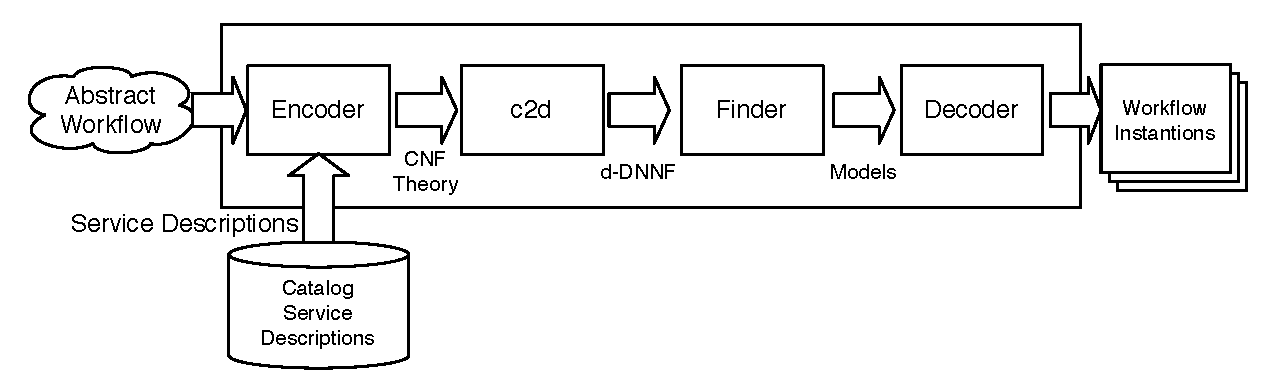
\includegraphics[width=.9\textwidth]{graphics/architecture}
\caption{Arquitectura del Sistema}
\label{fig:architecture}
\end{figure}

Se utiliza una arquitectura comprendida por un catálogo de descripciones de
servicio, el Codificador, el compilador c2d, el Buscador de mejores modelos, y
el Decodificador. La figura~\ref{fig:architecture} muestra la arquitectura global del sistema.
En esta infraestructura, una instancia del problema de instanciación de flujos
de trabajo se define como un flujo abstracto representado por una consulta
conjuntiva sobre servicios abstractos que es dada como entrada junto con un
conjunto de servicios concretos definidos por vistas de servicios abstractos.

El catálogo se pobla con descripciones de servicios abstractos y concretos; cada
servicio es descrito en términos de atributos de entrada y salida y anotado con
un valor real que representa la utilidad QoS del servicio. La descripción de los
servicios concretos, que son definidos como vistas de los servicios abstractos,
puede ser generada de manera semiautomática o automática usando herramientas
tales como el sistema DEIMOS \cite{AmbiteISWC09}.

Una instancia de entrada de WIP es codificada como una teoría CNF cuyos modelos
corresponden a las intanciaciones del flujo de trabajo por el Codificador. El
compilador c2d, un componente \emph{off-the-shelf}, compila la fórmula CNF a
d-DNNF. El Codificador traduce las instancias WIP en teorías CNF que luego son
convertidas en d-DNNF usando c2d. El Buscador computa un mejor modelo dados los
parámetros QoS en tiempo lineal en el tamaño del d-DNNF resultante. Es
importante remarcar que el proceso de compilación necesita ser realizado sólo
una vez ya que no depende del valor de los parámetros QoS. Así, incluso si la
compilación resulta ser costosa en términos de tiempo, este costo puede ser
amortizado dado que el d-DNNF resultante puede ser usado para conseguir mejores
instanciaciones con respecto a múltiples valores de los parámetros QoS.
Finalmente, el Decodificador traduce el mejor modelo retornado por el Buscador
a una instanciación de flujo de trabajo que resuelve el WIP.

Dado un CNF que codifica un WIP, su d-DNNF es una representación compacta de
todas las instanciaciones del flujo de trabajo. Es decir, uno puede generar de
una manera libre de \emph{backtracking} todas las instanciaciones del flujo de
trabajo. Si el usuario está interesado en una mejor instanciación dados
parámetros de QoS, entonces esta se puede computar en tiempo lineal en el tamaño
del d-DNNF. Si el usuario está interesado en todas las mejores instanciaciones,
estas pueden ser computadas en tiempo lineal en su número. Finalmente, si el
usuario está interesado en todas las instanciaciones, estas también pueden ser
computadas en tiempo lineal en su número. En los últimos dos casos, si ese
número es exponencial (en el tamaño de la entrada), la enumeración de las
instanciaciones también lo es pero esta complejidad es intrínsica al problema y
por lo tanto no puede ser evitada.

\subsection{Resultados Experimentales}

Se realizó un análisis empírico sobre tres experimentos. Todos los experimentos
fueron realizados en una máquina de escritorio con un CPU Intel Core 2 Duo de
2GHz y 4GB de memoria, y el tiempo fue medido con el comando de Unix
\emph{time}.

El objetivo de los experimentos es determinar el rendimiento de la propuesta con
condiciones variantes. El principal beneficio de la aproximación propuesta es
que se puede compilar la teoría lógica para una instancia del problema y luego
calcular todas las instanciaciones, o las mejores, cualquier número de veces. El
modelo de costos para conseguir mejores instanciaciones puede ser cambiado sin
necesidad de recompilar la teoría lógica. Por lo tanto, la complejidad en tiempo
de la aproximación es básicamente el tiempo para codificar el WIP como un
CNF más el tiempo para compilar el CNF en un d-DNNF y el tiempo para decodificar
los modelos. Los tiempos para codificar y decodificar son despreciables
comparados con el tiempo para compilar el CNF. Por esto, el enfoque es en el tiempo
necesario para compilar los problemas de los experimentos.

El primer experimento consiste de problemas para consultas para viajes aéreos.
Los servicios concretos son de la forma $V_i(x,y)\qrule\ \flight(x,y,\AL_i)$
donde $\AL_i$ es una
constante que denota el nombre de una aerolínea, y $\flight(x,y,\AL_i)$ relaciona las
ciudades $x$ e $y$ tales que hay un vuelo entre $x$ e $y$ servido por $\AL_i$.
Se supone que este servicio concreto retorna todos los vuelos entre dos ciudades
con una aerolínea específica. El flujo de trabajo tiene la forma

\[ W(x_1,\ldots,x_n)\ \qrule\ \flight(\PA,x_1,z),\,\flight(x_1,x_2,z),\,\ldots,\,\flight(x_n,\NY,z)\,. \]

\begin{figure}[t]
\centering
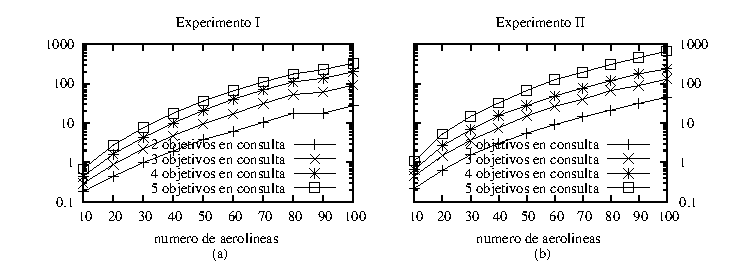
\includegraphics[width=1\textwidth]{graphics/plot1}
\caption{Tiempos de compilación para los experimentos I y II para diferentes
números de objetivos y de vistas. Los gráficos están en escala logarítmica, y el
tiempo es en segundos.}
\label{fig:plot1}
\end{figure}

El experimento incluye instancias para flujos de trabajo con 2 a 5 subobjetivos
y conjuntos de 10 a 100 servicios concretos. Los resultados para la compilación
son mostrados en el panel (a) de la figura ~\ref{fig:plot1}. Este es un gráfico en escala
logarítmica que sugiere comportamiento sub-exponencial. En cualquier caso, los
resultados muestran buen rendimiento dado que instancias realísticas del
problema (conjuntos de 100 aerolíneas con vuelos de cinco paradas) pueden ser
compiladas en 328 segundos. El tamaño en disco del d-DNNF para 100 aerolíneas y
vuelos con cinco paradas es 3,4MB. En este d-DNNF, el mejor modelo puede ser
computado en 0.29 segundos, y la enumeración de todos los modelos en 0.47
segundos.

En un intento de inducir crecimiento exponencial en el tamaño de compilación, en
el segundo experimento se agrega un segundo servicio concreto para cada
aerolínea. Esta modificación incrementa el número de instanciaciones válidas de
lineal a exponencial dado que cada tramo de un vuelo puede ser ahora instanciado
por dos servicios concretos y entonces un vuelo con $n$ tramos puede tener hasta
$2^n$ instanciaciones. Se corrió el compilador para instancias que comprendían
el mismo número de objetivos del flujo de trabajo y el número total de
servicios concretos. Los resultados graficados en escala logarítmica se muestran
en el panel (b) de la figura ~\ref{fig:plot1}.

Estas pruebas muestran buen rendimiento para este tipo de problemas, pero no
involucran servicios concretos con múltiples objetivos. Por lo tanto se
diseñó un tercer experimento que consiste de instancias no estructuradas y
generadas aleatoriamente. Cada instancia contiene tres variables por servicio
abstracto, diez variables distintas y diez constantes distintas, seis
objetivos en los flujos de trabajo, 2 a 5 objetivos en los servicios
concretos, y número de servicios variante. La probabilidad de que un argumento
de un servicio abstracto esté ligado a una constante es 50\%. Los resultados se
muestran en la figura ~\ref{fig:plot3}. El tiempo de compilación de estas instancias no
crece monótonamente dado que son generadas aleatoriamente. Lo mismo ocurre para
el tamaño de las teorías y los números de modelos. Por ejemplo, el d-DNNF para
un problema con 45 vistas cada una con 5 objetivos fue de tamaño 5,1Mb y tuvo
$1.26\times 10^8$ modelos. El tiempo para buscar el mejor modelo para este
d-DNNF es 0.46 segundos mientras que el tiempo para enumerar todos los modelos
es alredededor de 17 horas.

\begin{figure}[t]
\centering
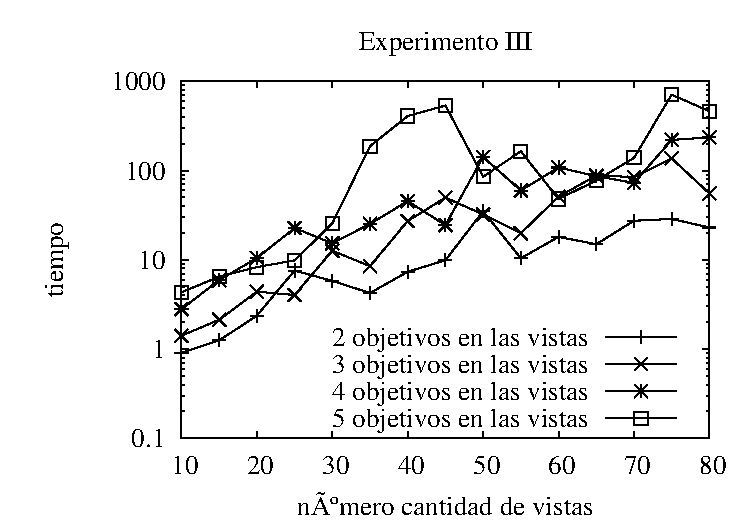
\includegraphics[width=.8\textwidth]{graphics/plot3}
\caption{Tiempos de compilación para el experimento III para diferentes números
de objetivos y de vistas. Los gráficos están en escala logarítmica, y el
tiempo es en segundos.}
\label{fig:plot3}
\end{figure}

Estos son experimentos preliminares, pero los resultados muestran que la
aproximación propuesta escala eficientemente para problemas con varios objetivos
y vistas. Se cree que estos resultados son alentadores y motivan a continuar
esta línea de investigación.
